\section{eo\-Expansion\-Mutation$<$ FType, Node $>$ Class Template Reference}
\label{classeo_expansion_mutation}\index{eoExpansionMutation@{eoExpansionMutation}}
eo\-Expansion\-Mutation --$>$ replace a terminal with a randomly created subtree  


{\tt \#include $<$gp/eo\-Parse\-Tree\-Op.h$>$}

Inheritance diagram for eo\-Expansion\-Mutation$<$ FType, Node $>$::\begin{figure}[H]
\begin{center}
\leavevmode
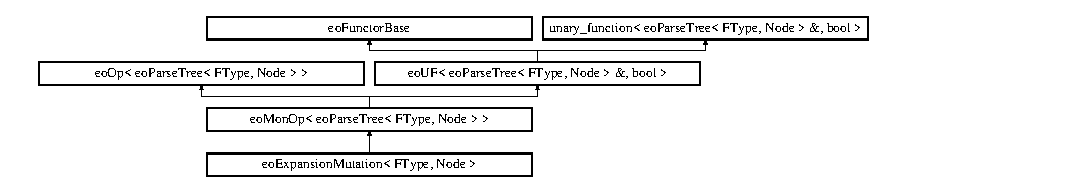
\includegraphics[height=2.14559cm]{classeo_expansion_mutation}
\end{center}
\end{figure}
\subsection*{Public Types}
\begin{CompactItemize}
\item 
typedef {\bf eo\-Parse\-Tree}$<$ FType, Node $>$ {\bf Eo\-Type}\label{classeo_expansion_mutation_w0}

\end{CompactItemize}
\subsection*{Public Member Functions}
\begin{CompactItemize}
\item 
{\bf eo\-Expansion\-Mutation} ({\bf eo\-Init}$<$ {\bf Eo\-Type} $>$ \&\_\-init, unsigned \_\-max\_\-length)
\begin{CompactList}\small\item\em Constructor. \item\end{CompactList}\item 
virtual std::string {\bf class\-Name} () const \label{classeo_expansion_mutation_a1}

\begin{CompactList}\small\item\em The class name. \item\end{CompactList}\item 
virtual {\bf $\sim$eo\-Expansion\-Mutation} ()\label{classeo_expansion_mutation_a2}

\begin{CompactList}\small\item\em Dtor. \item\end{CompactList}\item 
bool {\bf operator()} ({\bf Eo\-Type} \&\_\-eo1)
\begin{CompactList}\small\item\em Mutate an individual. \item\end{CompactList}\end{CompactItemize}
\subsection*{Private Attributes}
\begin{CompactItemize}
\item 
unsigned {\bf max\_\-length}\label{classeo_expansion_mutation_r0}

\item 
{\bf eo\-Init}$<$ {\bf Eo\-Type} $>$ \& {\bf initializer}\label{classeo_expansion_mutation_r1}

\end{CompactItemize}


\subsection{Detailed Description}
\subsubsection*{template$<$class FType, class Node$>$ class eo\-Expansion\-Mutation$<$ FType, Node $>$}

eo\-Expansion\-Mutation --$>$ replace a terminal with a randomly created subtree 



Definition at line 204 of file eo\-Parse\-Tree\-Op.h.

\subsection{Constructor \& Destructor Documentation}
\index{eoExpansionMutation@{eo\-Expansion\-Mutation}!eoExpansionMutation@{eoExpansionMutation}}
\index{eoExpansionMutation@{eoExpansionMutation}!eoExpansionMutation@{eo\-Expansion\-Mutation}}
\subsubsection{\setlength{\rightskip}{0pt plus 5cm}template$<$class FType, class Node$>$ {\bf eo\-Expansion\-Mutation}$<$ FType, Node $>$::{\bf eo\-Expansion\-Mutation} ({\bf eo\-Init}$<$ {\bf Eo\-Type} $>$ \& {\em \_\-init}, unsigned {\em \_\-max\_\-length})\hspace{0.3cm}{\tt  [inline]}}\label{classeo_expansion_mutation_a0}


Constructor. 

\begin{Desc}
\item[Parameters:]
\begin{description}
\item[{\em \_\-init}]An instantiation of eo\-Gp\-Depth\-Initializer \item[{\em \_\-max\_\-length}]the maximum size of an individual \end{description}
\end{Desc}


Definition at line 215 of file eo\-Parse\-Tree\-Op.h.

\subsection{Member Function Documentation}
\index{eoExpansionMutation@{eo\-Expansion\-Mutation}!operator()@{operator()}}
\index{operator()@{operator()}!eoExpansionMutation@{eo\-Expansion\-Mutation}}
\subsubsection{\setlength{\rightskip}{0pt plus 5cm}template$<$class FType, class Node$>$ bool {\bf eo\-Expansion\-Mutation}$<$ FType, Node $>$::operator() ({\bf Eo\-Type} \& {\em \_\-eo1})\hspace{0.3cm}{\tt  [inline]}}\label{classeo_expansion_mutation_a3}


Mutate an individual. 

\begin{Desc}
\item[Parameters:]
\begin{description}
\item[{\em \_\-eo1}]The individual that is to be changed \end{description}
\end{Desc}


Definition at line 228 of file eo\-Parse\-Tree\-Op.h.

References eo\-Parse\-Tree$<$ FType, Node $>$::prune\-Tree(), and eo\-Rng::random().

The documentation for this class was generated from the following file:\begin{CompactItemize}
\item 
eo\-Parse\-Tree\-Op.h\end{CompactItemize}
